\documentclass[12pt]{article}
\usepackage{amssymb,amsmath,graphicx,mathtools}
\usepackage{listings}
\usepackage[margin=0.75in]{geometry}
\parindent 16 pt
\usepackage{fancyhdr}
\pagestyle{fancy}
\fancyhead[R]{Swupnil Sahai}
\fancyhead[L]{Square Root Hierarchical Model}
\DeclarePairedDelimiter\ceil{\lceil}{\rceil}
\DeclarePairedDelimiter\floor{\lfloor}{\rfloor}

\lstset{
    language=R,
    basicstyle=\scriptsize\ttfamily,
    stepnumber=1,
    numbersep=5pt,
    showspaces=false,
    showstringspaces=false,
    showtabs=false,
    frame=single,
    tabsize=2,
    captionpos=b,
    breaklines=true,
    breakatwhitespace=false,
    escapeinside={},
    keywordstyle={},
    morekeywords={}
    }

\begin{document}

% CUSTOM SHORTCUTS

\def\ci{\perp\!\!\!\perp}
\def\ex{\mathbb{E}}
\def\prob{\mathbb{P}}
\def\ind{\mathbb{I}}
\def\grad{\triangledown}
\def\bigo{\mathcal{O}}

\section{General Model Framework}
We wish to split the sky map into longitudinal bins, regressing FUV ($y_{ij}$) on i100 ($x_{ij}$) within each bin $i$. As such, this problem lends itself to a hierarchical framework in which each longitudinal bin has its own slope $\beta_{1i}$ and intercept $\beta_{0i}$, where all of the slopes and intercepts are drawn from common prior distributions. This can be represented graphically as:\\

\indent\indent\indent\indent\indent\indent\indent\indent 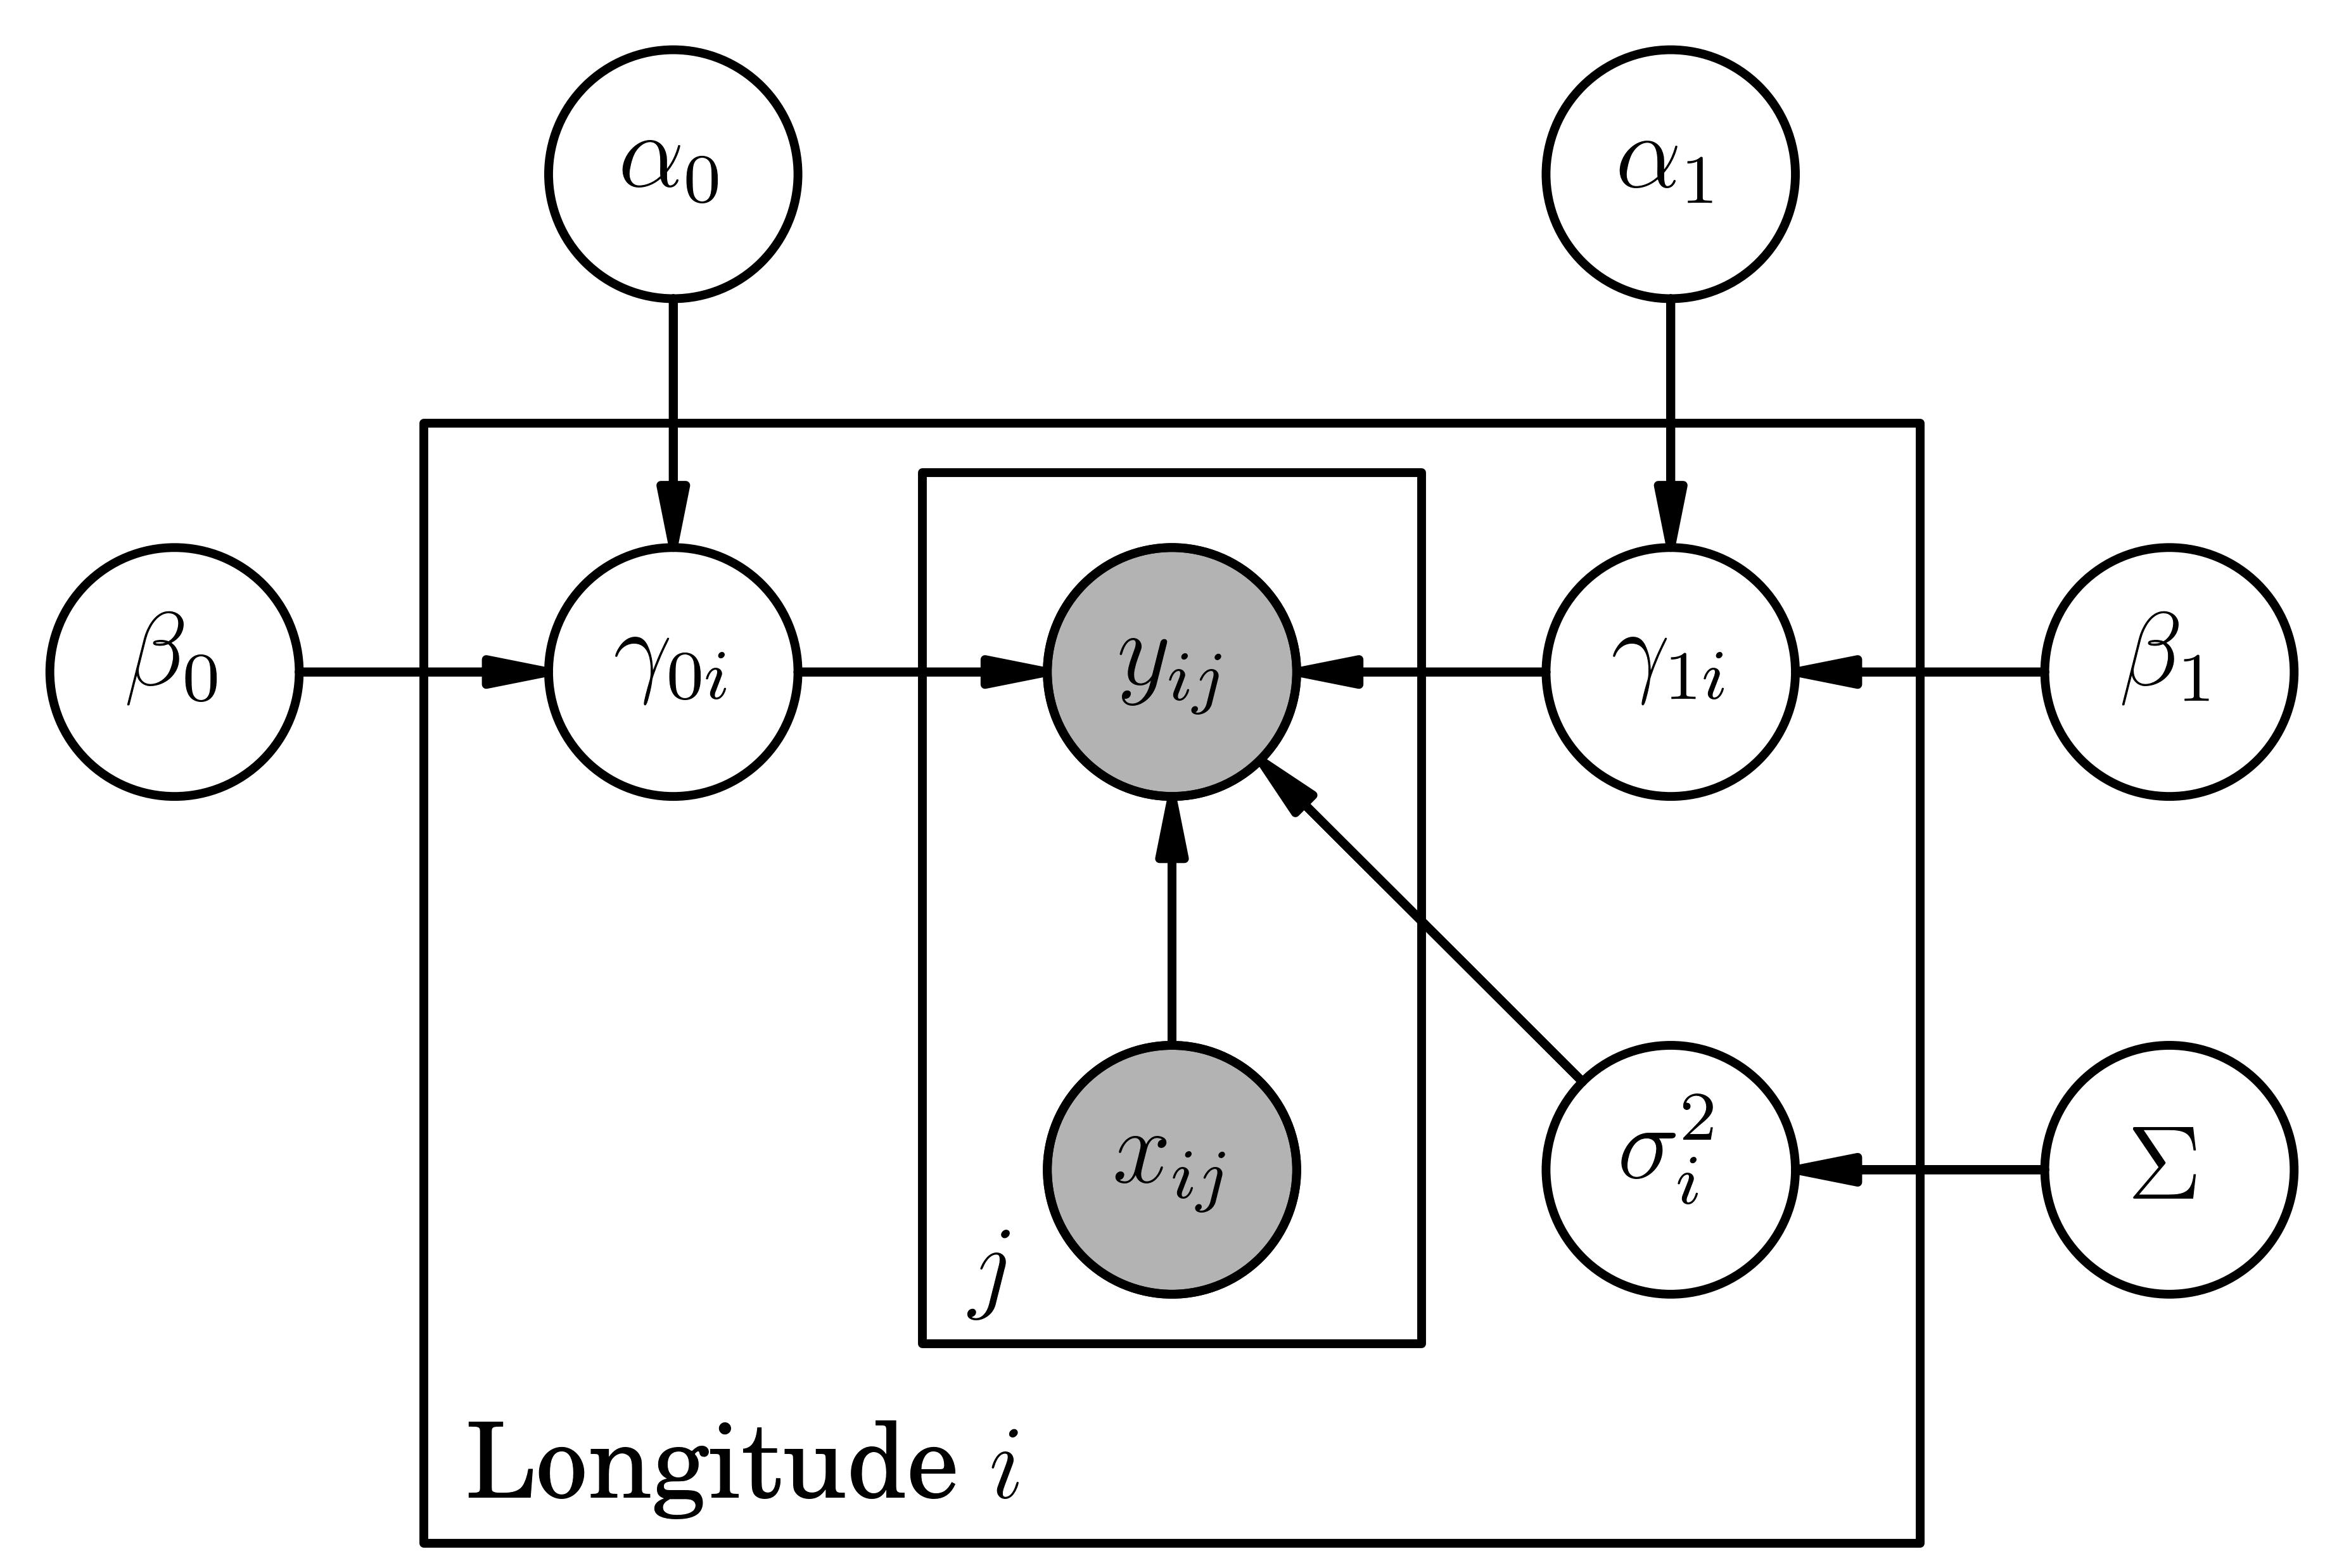
\includegraphics{SquareRoot_Model.png}

\subsection{Square Root Model}
We model $y_{ij}$ as a square root function of the strictly positive parameters with the following setup:
$$y_{ij} \sim N \biggl( \sqrt{ \beta_{0i}^2 + \beta_{1i}^2 x_{ij}^2} , \sigma_i^2 \biggr)
\hspace{20 pt} \beta_{0i} \sim N(\mu_0,\tau_0^2)
\hspace{20 pt} \beta_{1i} \sim N(\mu_1,\tau_1^2)
\hspace{20 pt} \log\sigma_i \sim N(\mu_\sigma,\tau_\sigma^2)$$

\subsection{Linear Model}
An alternative setup is to consider $y_{ij}$ as a linear function of the strictly positive parameters:
$$y_{ij} \sim N \biggl( \beta_{0i} + \beta_{1i} x_{ij} , \sigma_i^2 \biggr)
\hspace{20 pt} \beta_{0i} \sim N(\mu_0,\tau_0^2)
\hspace{20 pt} \beta_{1i} \sim N(\mu_1,\tau_1^2)
\hspace{20 pt} \log\sigma_i \sim N(\mu_\sigma,\tau_\sigma^2)$$

\subsection{Adjusted Linear Model}
In an attempt to shrink $\beta_0$ closer to 0, we could model $y_{ij}$ as a linear function of $\sqrt{x_{ij}}$:
$$y_{ij} \sim N \biggl( \beta_{0i} + \beta_{1i} \sqrt{x_{ij}} , \sigma_i^2 \biggr)
\hspace{20 pt} \beta_{0i} \sim N(\mu_0,\tau_0^2)
\hspace{20 pt} \beta_{1i} \sim N(\mu_1,\tau_1^2)
\hspace{20 pt} \log\sigma_i \sim N(\mu_\sigma,\tau_\sigma^2)$$

\subsection{No Intercept Linear Model}
Lastly, to guarantee $\beta_0 = 0$, we can model $y_{ij}$ without an intercept term altogether:
$$y_{ij} \sim N \biggl( \beta_{1i} x_{ij} , \sigma_i^2 \biggr)
\hspace{20 pt} \beta_{1i} \sim N(\mu_1,\tau_1^2)
\hspace{20 pt} \log\sigma_i \sim N(\mu_\sigma,\tau_\sigma^2)$$

%SUMMARY
\pagebreak
\section{Summary of Results}
To see a quick comparison of all of the results, the following tables are helpful.
\subsection{Parameters}
I fit each model in Stan using 36 longitudinal bins and sampling 100 data points from each bin, with 4 chains of 1000 iterations. The posterior means of the parameters are shown in the following table.
\begin{table}[ht]
\caption{Posterior Mean of Hyperparameters}
\centering
\begin{tabular}{c c c c c c c c}
\hline\hline
$y$ & Run Time (Min.) & $\mu_0$ & $\tau_0$ & $\mu_1$ & $\tau_1$ & $\mu_\sigma$ & $\tau_\sigma$ \\ [0.5ex] % inserts table %heading
\hline \\
$\sqrt{\beta_0^2+\beta_1^2x^2}$ & 2.26 & 427.01 & 151.72 & 275.52 &  102.93 & 6.15 &  0.29 \\
$\beta_0+\beta_1x$ & 1.28 & 270.31 & 160.61 & 248.90 & 108.69 & 6.13 &  0.29\\
$\beta_0+\beta_1\sqrt{x}$ & 3.01 & 2.20 & 0.69 & 683.70 & 116.41 & 6.27 & 0.33\\
$\beta_1x$ & 2.12 & 0 & 0 & 293.68 & 97.70 & 6.23 &  0.26\\ 
\hline
\end{tabular}
\label{table:nonlin}
\end{table}

\subsection{Correlation With Light Intensity}
Since the $x$ and $y$ were grouped into 36 longitudinal bins, I took the light intensity metrics (there were 360 observations for each metric) and simply took the averages of the metrics across each of the 36 longitudinal bins. I then evaluated the correlation between slope / intercept and each light intensity metric. This was repeated for each model.
\begin{table}[ht]
\caption{Correlation of Slope $(\beta_1)$}
\centering
\begin{tabular}{c c c c c }
\hline\hline
$y$ & $1e6 N$ & $1e6 S$ & $1e5 N$ & $1e5 S$\\ [0.5ex] % inserts table %heading
\hline \\
$\sqrt{\beta_0^2+\beta_1^2x^2}$ & 0.11 & -0.15 & -0.023 &  -0.43 \\
$\beta_0+\beta_1x$ & 0.14 & -0.19 & -0.0079 & -0.46 \\
$\beta_0+\beta_1\sqrt{x}$ & 0.19 & -0.23 & 0.046 & -0.39\\
$\beta_1x$ & 0.079 & -0.10 & -0.045 & -0.39 \\ 
\hline
\end{tabular}
\label{table:nonlin}
\end{table}

\begin{table}[ht]
\caption{Correlation of Intercept $(\beta_0)$}
\centering
\begin{tabular}{c c c c c }
\hline\hline
$y$ & $1e6 N$ & $1e6 S$ & $1e5 N$ & $1e5 S$\\ [0.5ex] % inserts table %heading
\hline \\
$\sqrt{\beta_0^2+\beta_1^2x^2}$ & -0.17 & 0.25 & -0.026 &  0.54 \\
$\beta_0+\beta_1x$ & -0.26 & 0.21 & -0.076 & 0.57 \\
$\beta_0+\beta_1\sqrt{x}$ & 0.049 & -0.029 & -0.10 & 0.079\\
\hline
\end{tabular}
\label{table:nonlin}
\end{table}

\noindent More detailed plots of the parameters versus longitude as well as plots of the slope/intercept versus the light intensity metrics can be found on the remaining pages. 

%SQUARE ROOT MODEL FITTING
\pagebreak
\section{Square-Root Model Fitting}
I fit the hierarchical square-root model in Stan using 36 longitudinal bins and sampling 100 data points from each bin, with 4 chains of 1000 iterations (Total Run Time: 2.26 Minutes).  The posterior means of all of the parameters, versus longitude, are shown below:

\indent\indent 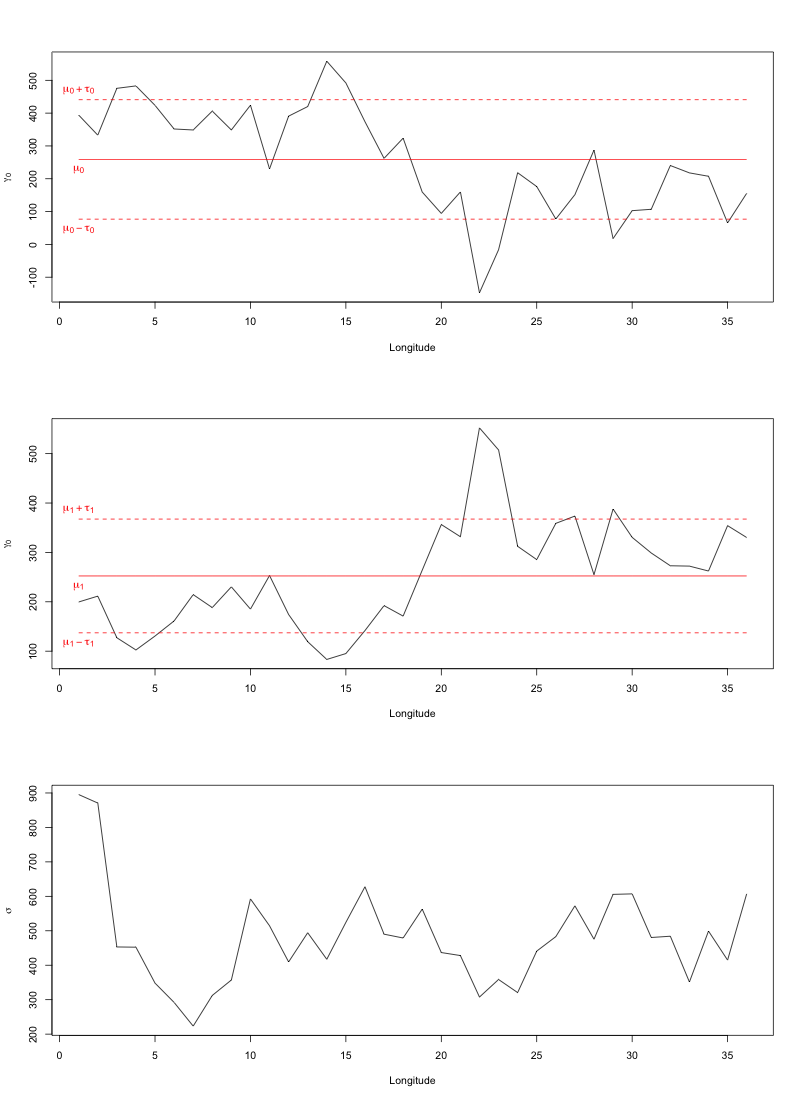
\includegraphics[scale=0.55]{params.png}

\pagebreak
\subsection{Relationship With Star Light Intensity}

\subsubsection{Slope Versus Light Intensity}
It seems that for the square root model, the slope only has a moderately high correlation with the FUV 1e5 S metric.\\
\indent\indent 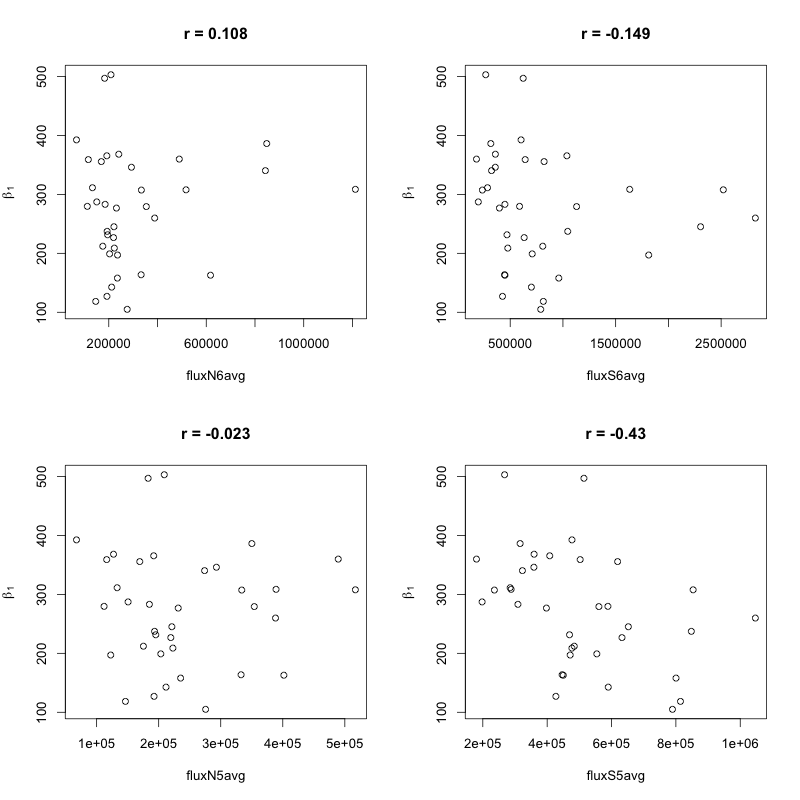
\includegraphics[scale=0.55]{flux_v_b1.png}

\subsubsection{Intercept Versus Light Intensity}
The intercept, similarly, has a moderately high correlation with the FUV 1e5 S metric.\\
\indent\indent 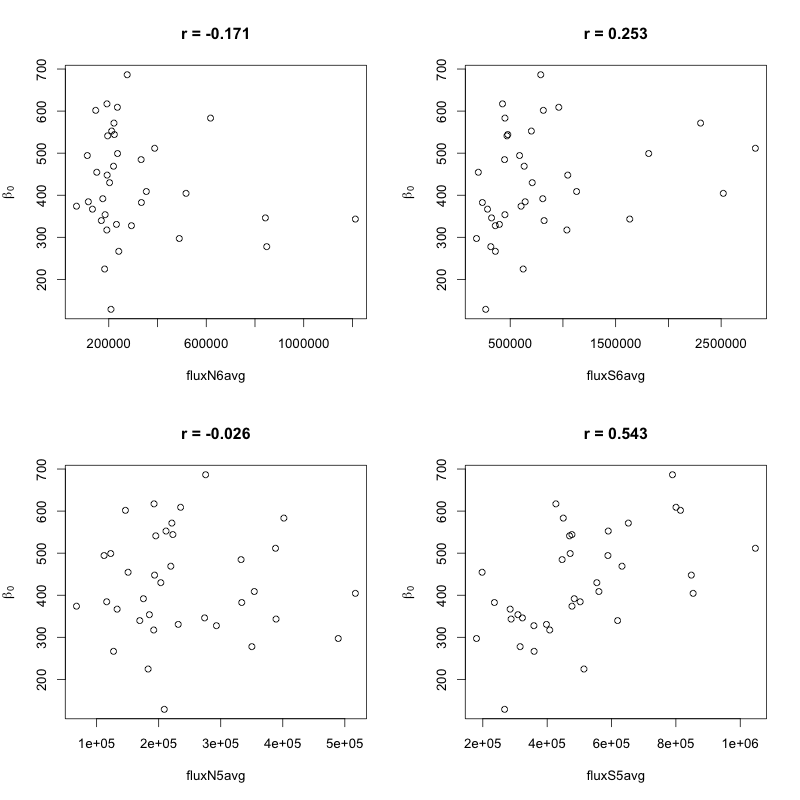
\includegraphics[scale=0.55]{flux_v_b0.png}

%LINEAR MODEL FITTING
\pagebreak
\section{Linear Model Fitting}
I also fit the standard linear model in Stan using 36 longitudinal bins and sampling 100 data points from each bin, with 4 chains of 1000 iterations (Total Run Time: 1.28 Minutes).  The posterior means of all of the parameters are shown below:

\indent\indent 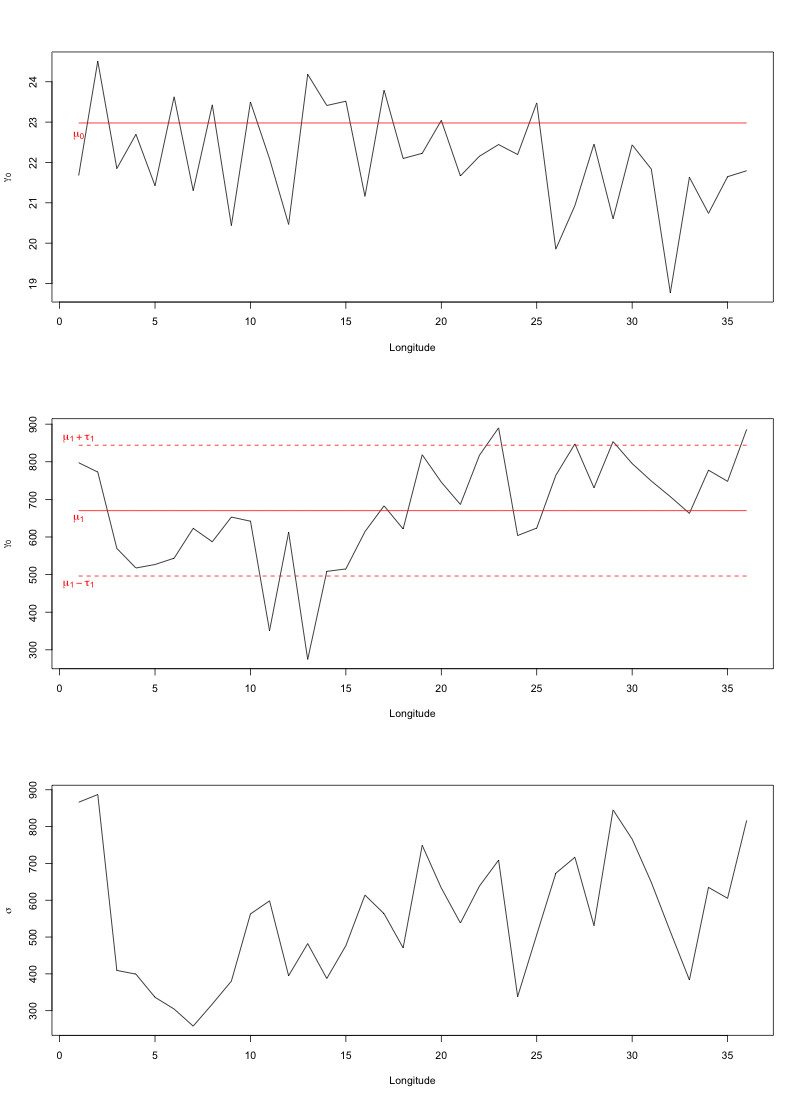
\includegraphics[scale=0.55]{params2.png}

\pagebreak
\subsection{Relationship With Star Light Intensity}

\subsubsection{Slope Versus Light Intensity}
The correlations for the slope are higher in the linear model than they were in the square root model, except for the FUV 1e5 S metric.\\
\indent\indent 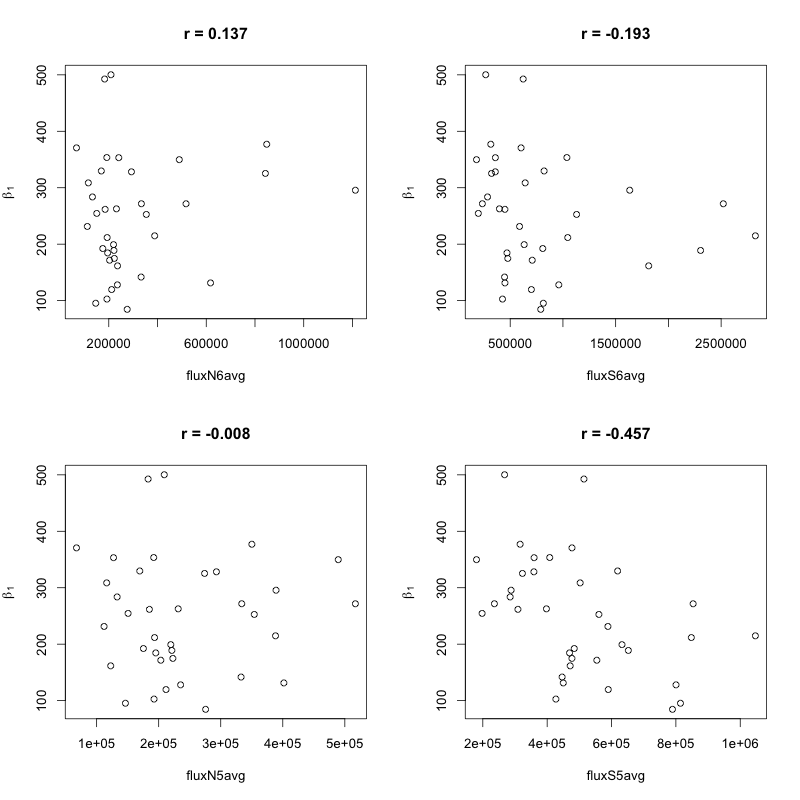
\includegraphics[scale=0.55]{flux_v_b1_2.png}

\pagebreak
\subsubsection{Intercept Versus Light Intensity}
The intercept for the linear model has has higher correlation than the square-root model, across all flux metrics.\\
\indent\indent 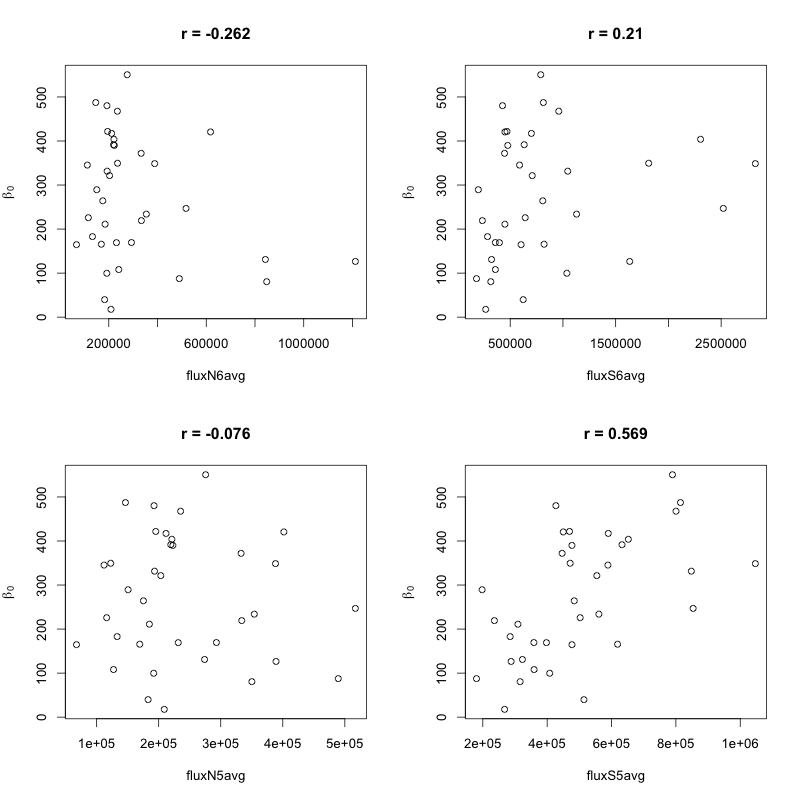
\includegraphics[scale=0.55]{flux_v_b0_2.png}

%ADJUSTED LINEAR MODEL FITTING
\pagebreak
\section{Adjusted Linear Model Fitting}
I lastly fit the adjusted linear model in Stan using 36 longitudinal bins and sampling 100 data points from each bin, with 4 chains of 1000 iterations (Total Run Time: 3.01 Minutes).  The posterior means of all of the parameters are shown below:

\indent\indent 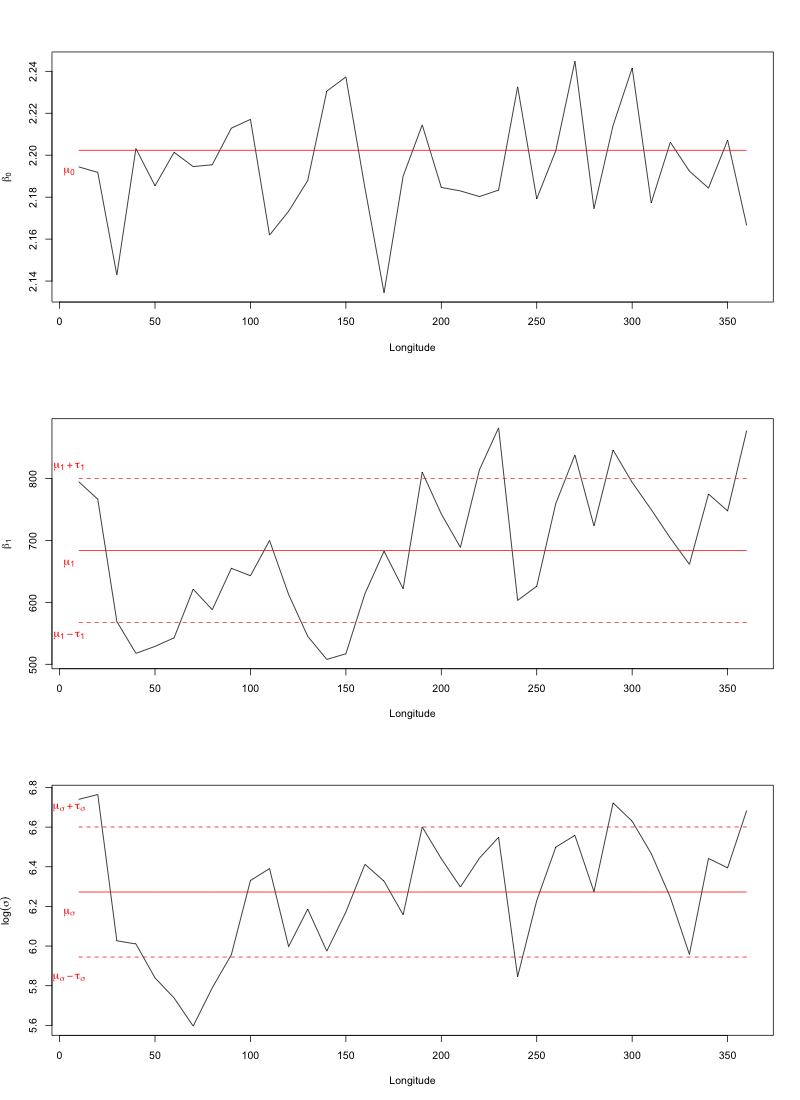
\includegraphics[scale=0.55]{params1.png}

\pagebreak
\subsection{Relationship With Star Light Intensity}

\subsubsection{Slope Versus Light Intensity}
The correlations for the slope are higher in the adjusted linear model than they were in the square root model or the standard linear model, except for correlation with FUV 1e5 S metric.\\
\indent\indent 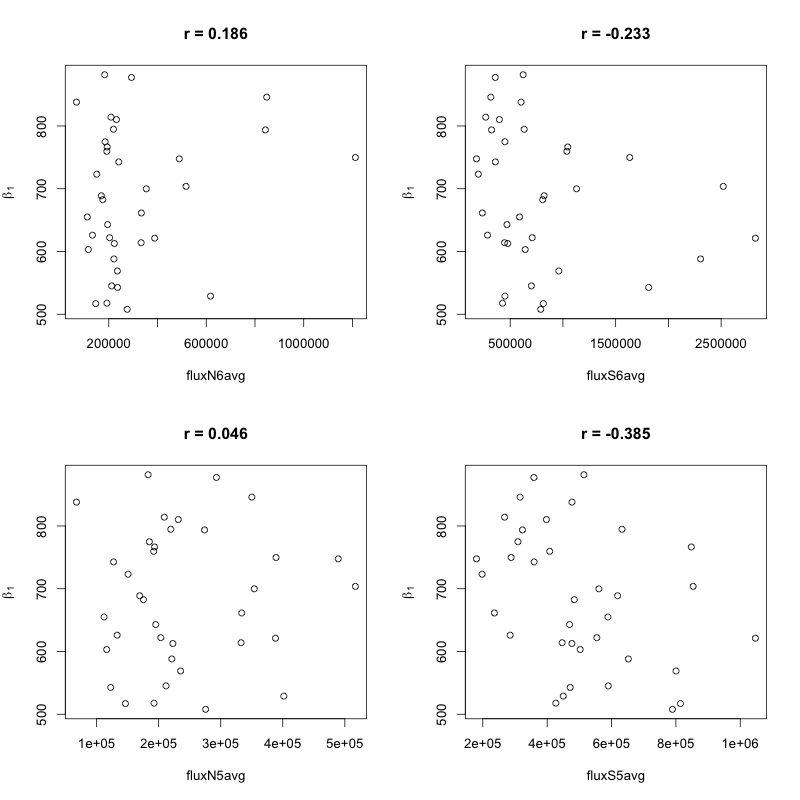
\includegraphics[scale=0.55]{flux_v_b1_1.png}

\pagebreak
\subsubsection{Intercept Versus Light Intensity}
The intercept for the adjusted linear model has more even correlation across the flux metrics, and the high correlation with FUV 1e5 S has decreased compared to the correlation of the square root model's intercept with this same metric.\\
\indent\indent 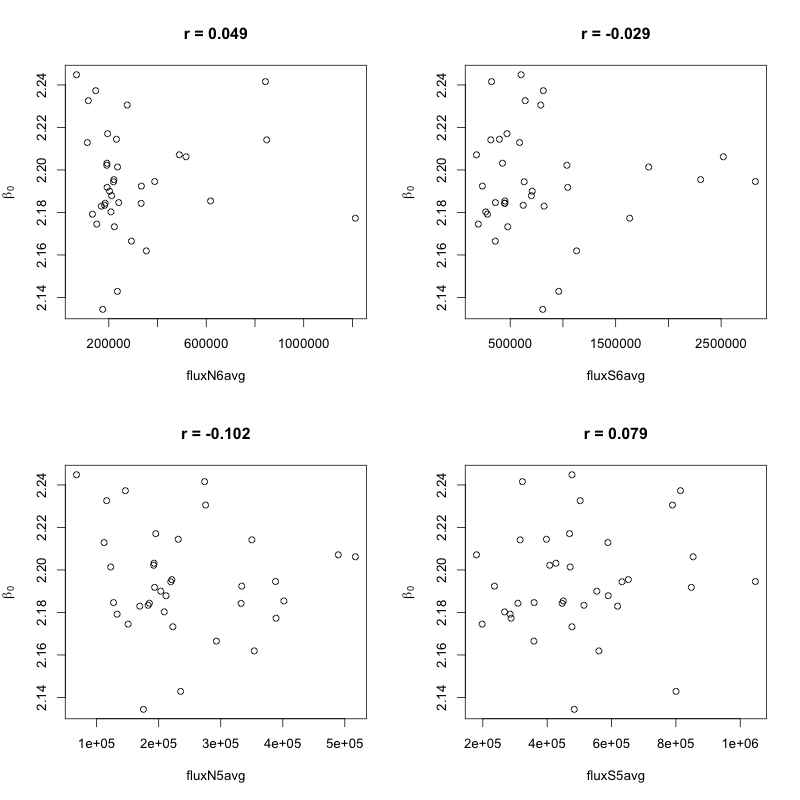
\includegraphics[scale=0.55]{flux_v_b0_1.png}

%NO INTERCEPT LINEAR MODEL FITTING
\pagebreak
\section{No Intercept Linear Model Fitting}
I lastly fit the adjusted linear model in Stan using 36 longitudinal bins and sampling 100 data points from each bin, with 4 chains of 1000 iterations (Total Run Time: 2.12 Minutes).  The posterior means of all of the parameters are shown below:

\indent\indent 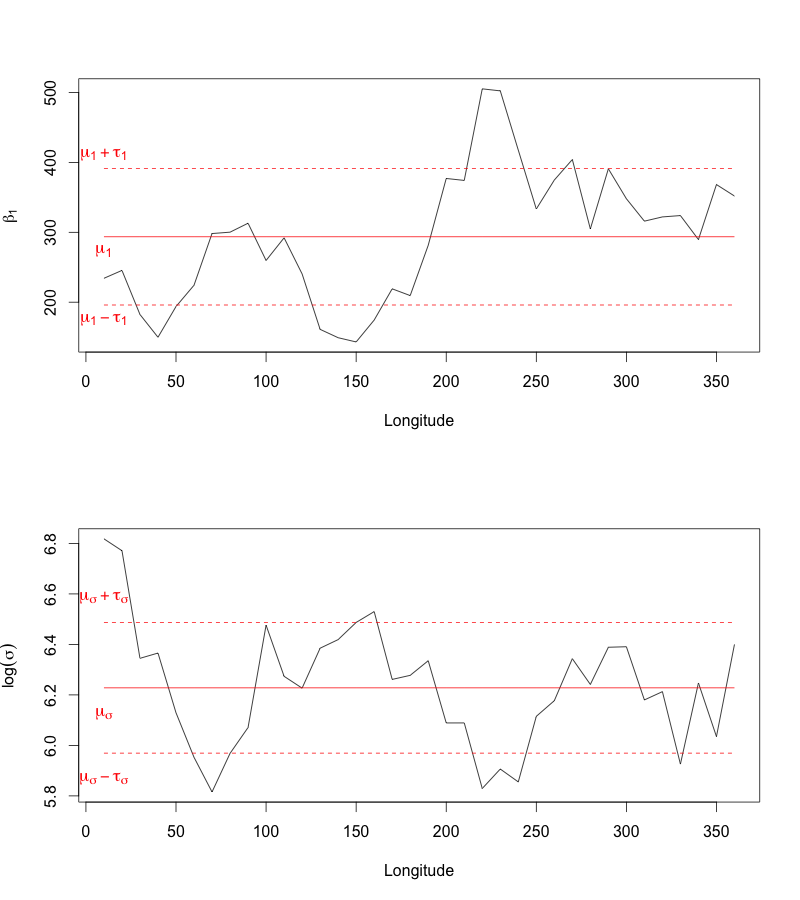
\includegraphics[scale=0.55]{params3.png}

\pagebreak
\subsubsection{Slope Versus Light Intensity}
The correlations for the slope are slightly lower in the no-intercept linear model than they were in the adjusted linear model.\\
\indent\indent 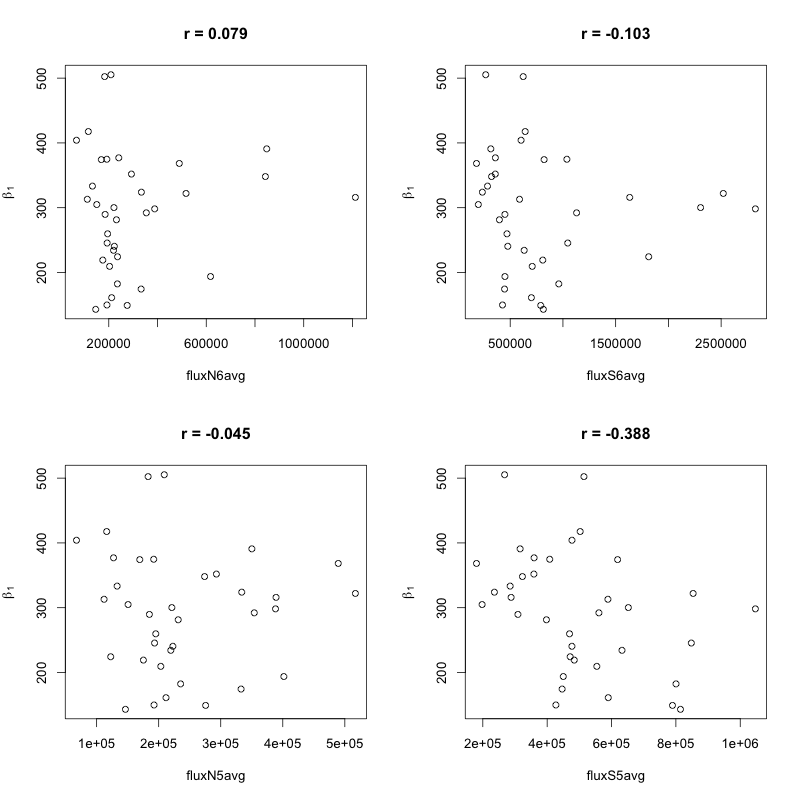
\includegraphics[scale=0.55]{flux_v_b1_3.png}

%CODE
%\pagebreak
%\section{Code}
%\texttt{\lstinputlisting{hierarchical_model.R}}

\end{document}